% $Header: /home/vedranm/bitbucket/beamer/solutions/generic-talks/generic-ornate-15min-45min.en.tex,v 90e850259b8b 2007/01/28 20:48:30 tantau $

\documentclass{beamer}

% This file is a solution template for:

% - Giving a talk on some subject.
% - The talk is between 15min and 45min long.
% - Style is ornate.



% Copyright 2004 by Till Tantau <tantau@users.sourceforge.net>.
%
% In principle, this file can be redistributed and/or modified under
% the terms of the GNU Public License, version 2.
%
% However, this file is supposed to be a template to be modified
% for your own needs. For this reason, if you use this file as a
% template and not specifically distribute it as part of a another
% package/program, I grant the extra permission to freely copy and
% modify this file as you see fit and even to delete this copyright
% notice. 


\mode<presentation>
{
  \usetheme{Warsaw}
  % or ...

  \setbeamercovered{transparent}
  % or whatever (possibly just delete it)
}


\usepackage[english]{babel}
% or whatever

\usepackage[latin1]{inputenc}
% or whatever

\usepackage{times}
\usepackage[T1]{fontenc}
% Or whatever. Note that the encoding and the font should match. If T1
% does not look nice, try deleting the line with the fontenc.


\title[MRes Advanced Brain Imaging] % (optional, use only with long paper titles)
{MRes Advanced Brain Imaging}

\subtitle[Revision session]
{Revision session} % (optional)

\author[Remi Gau] % (optional, use only with lots of authors)
{Remi Gau}

\institute[University of Birmingham] % (optional, but mostly needed)
{
  School of psychology\\
  University of Birmingham
}

\date[Short Occasion] % (optional)
{11\textsuperscript{th} February 2013}

\subject{MRes Advanced Brain Imaging - Revision session}
% This is only inserted into the PDF information catalog. Can be left
% out. 



% If you have a file called "university-logo-filename.xxx", where xxx
% is a graphic format that can be processed by latex or pdflatex,
% resp., then you can add a logo as follows:
\pgfdeclareimage[height=0.5cm]{university-logo}{university-logo-filename.jpeg}
\logo{\pgfuseimage{university-logo}}



% If you wish to uncover everything in a step-wise fashion, uncomment
% the following command: 
%\beamerdefaultoverlayspecification{<+->}


\begin{document}

\footnotesize


\begin{frame}
  \titlepage
\end{frame}

%----------------------------------------------------------------------------------------------------------------------------------------------------------
%----------------------------------------------------------------------------------------------------------------------------------------------------------

\section{PRE-PROCESSING}

%----------------------------------------------------------------------------------------------------------------------------------------------------------

\subsection[General questions]{General questions}

% \begin{frame}{General questions}
%   \begin{itemize}
%   \item How do you map from voxel space to MNI space?
%     transformation matrix : rotation, translation, scaling
%     MNI : 0 0 0 is the AC
%   \end{itemize}
% \end{frame}


\begin{frame}{General questions}
  \begin{itemize}
    \item \textbf{What is an objective function when comparing 2 images?}
  
\smallskip 
It is a function that allows quantification of the difference between these images and the optimization of the parameters set to get their best realignment, usually by minimizing/maximizing its value.

\bigskip
  \item \textbf{Why are there different objective functions?}
  
\smallskip   
T1 and T2 weighted have very different ranges of values for the same tissue class.
  \end{itemize}
\end{frame}


\begin{frame}{General questions}
\textbf{Which objective functions are used for (1) realignment of functional images and (2) coregistration of a structural and functional image? }

\smallskip    
    \begin{enumerate}
     
     \item Realignment : within modality
      \begin{itemize}\footnotesize
	\item Least squares : minimize
	\item Normalized cross correlation : maximize
      \end{itemize}
      
     \item Registration : between modality (usually entropy based approaches)
      \begin{itemize}\footnotesize
	\item Mutual information : maximize
	\item Normalized Mutual information : maximize
      \end{itemize}     
    \end{enumerate} 
\end{frame}


\begin{frame}{General questions}
\textbf{If you resample your images after each preprocessing step, how will the images look different (as compared to when you resampled only after smoothing)?}

\smallskip  
Your images will be smoother : interpolation error increases the smoothness of your data.

\end{frame}

%----------------------------------------------------------------------------------------------------------------------------------------------------------

\subsection[Slice timing]{Slice timing}

\begin{frame}{Slice timing}
In their simulation data, Sladky et al. (2011) found that to slice-delay effects were more pronounced for experimental designs long TRs (4 secs) compare to short TRs (1 secs), or for event-related and short block designs (10 secs) compared to long blocks (30 secs) design.

\smallskip
\textbf{Can you explain those results?}

\smallskip    
  \begin{itemize}
      \item Longer TRs are more affected because more time goes by between the first and and last acquired slices.
      \item Event related and short blocks are more affected because there will be quicker temporal changes in the the BOLD signal.
  \end{itemize}


\end{frame}

%----------------------------------------------------------------------------------------------------------------------------------------------------------

\subsection[Realignment]{Realignment}

\begin{frame}{Realignment}
\textbf{What are some the possible sources of residual errors that are still present after realignment?}

\smallskip 
    \begin{enumerate}
      \item Re-sampling can introduce interpolation errors
      \item Gaps between slices can cause aliasing artifacts
      \item Slices are not acquired simultaneously: rapid movements not accounted for by rigid body model
      \item Image artifacts may not move according to a rigid body model
      \begin{itemize}\footnotesize
	  \item image distortion and realignment $\times$ inhomogeneity interaction
	  \item image dropout
	  \item Nyquist ghost
      \end{itemize}
      \item Spin history effect: Motion can also alter the MR signal because protons that moves into a voxel from a neighbouring slice have an excitation different from that expected by the scanner and the signal will not reflect well the tissue in that voxel. This spin history effect is not corrected using motion correction algorithms and Independent Component Analysis (ICA) or dedicated methods must be used.

    \end{enumerate}  
\end{frame}


\begin{frame}{Realignment}
\textbf{What can you do to minimize the effects of those residual errors?}

\smallskip 
    \begin{enumerate}
      \item Unwarp your data (if you have not already done so).
      \item Include realignment parameters in the design matrix of your GLM.
    \end{enumerate}  
\end{frame}

%----------------------------------------------------------------------------------------------------------------------------------------------------------

\subsection[normalization]{normalization}

\begin{frame}{Normalization}
\textbf{What are the reasons for normalization?}

\smallskip 
    \begin{enumerate}
      \item Try to account for inter-subject anatomical variability
      \item Express results in a standard common space across studies
    \end{enumerate}
\end{frame}    


\begin{frame}{Normalization}
After acquiring one anatomical and a series of functional images, you want to normalize all the images. \textbf{Describe two distinct processing streams that would bring the images of both modalities into a standard (e.g. MNI) space. What are the (dis)advantages of the two streams?}

\smallskip 
    \begin{enumerate}
      \item T1 images normalized to T1 template and EPI images to the EPI template: less accurate as the lower resolution of the EPI images will mean that the registration will be driven by high-contrast feature of the brain (e.g edges)
      \item Coregister the mean EPI and structural images, segment the structural image (GM/WM/CSF) which implies a normalization step and will produce normalization parameters that can then be used to normalize the EPI images. The inconvenient of this stream is that some of the distortion specific to EPI images might not be accounted for.
    \end{enumerate}
\end{frame}
    
    
\begin{frame}{Normalization}
\textbf{Most spatial normalization procedures involves two steps, affine and non-linear transformation. Why?}
    
\smallskip     
    \begin{enumerate}
      \item Affine : rigid body transformation (3 translations & 3 rotations) & sheers & scalings
      \item Non-linear : warping for better match between structures
    \end{enumerate}    
\end{frame}

\begin{frame}{Normalization}
\textbf{What alternatives are there if you still want to average results accross subjects without normalising your data?}
    
\smallskip     
    \begin{enumerate}
      \item Using some clear anatomical features to define a region of interest, but this requires some anatomical expertise and involves even when performed by experts involves some criterion that are hard to operationalize. 
      \item Using functional localizer to define a functional region of interest within which the average will be done.
    \end{enumerate}    
\end{frame}

%----------------------------------------------------------------------------------------------------------------------------------------------------------

\subsection[Smoothing]{Smoothing}

\begin{frame}{Smoothing}
  \begin{itemize}  
    \item \textbf{What are the main reasons for spatial smoothing ?}
  
\smallskip 
    \begin{enumerate}\footnotesize
      \item Compensate for inter-subject variability
      \item Matched filter theorem
      \item Sufficient smoothness of the data is necessary if random field theory has to be used for multiple comparison
    \end{enumerate}

\bigskip
    \item \textbf{What is the matched filter theorem?}

\smallskip   
Using a filter that has the same shape as the signal will give the best signal to noise ratio. 

\bigskip
    \item \textbf{If we expect your signal to be of Gaussian shape with a kernel of 8 mm FWHM, which smoothing kernel would you use?}

\smallskip   
A gaussian shape with a kernel of 8 mm FWHM.
    
  \end{itemize}
\end{frame}

%----------------------------------------------------------------------------------------------------------------------------------------------------------
%----------------------------------------------------------------------------------------------------------------------------------------------------------

\section{GENERAL LINEAR MODEL}

\subsection[General questions]{General questions}


\begin{frame}{General questions}
\textbf{Draw a Venn diagram of: t-test, paired t-test, ANOVA, repeated measures ANOVA, General Linear model.}

\smallskip
    \begin{center}
      \includegraphics[scale=0.5,keepaspectratio=true]{./Venn_GLM.jpg}
      % Venn_GLM.jpg: 1540x1007 pixel, 299dpi, 13.08x8.55 cm, bb=0 0 371 242
    \end{center}
\end{frame} 


\begin{frame}{General questions}
\textbf{If two regressors X$_{1}$ and X$_{2}$ are correlated, what do the $\beta$ estimates represent?}

\smallskip 
Only the variability unique to a regressor drives the parameter estimate of that regressor.

\smallskip
    \begin{center}
      \includegraphics[scale=0.6,keepaspectratio=true]{./CorrelatedRegressors.jpg}
      % CorrelatedRegressors.jpg: 922x727 pixel, 299dpi, 7.83x6.18 cm, bb=0 0 222 175
    \end{center}
\end{frame} 


\begin{frame}{General questions}
\textbf{If regressor 1 and 2 are correlated and you orthogonalize 2 with respect to 1 which, if any, $\beta$ will change and why? Explain via geometric perspective.}
  
\smallskip   
The $\beta$ associated to the regressor 1 will change.

\smallskip  
    \begin{flushleft}
    \includegraphics[scale=0.27,keepaspectratio=true]{./Ortho_And_Non-Ortho_Regressors.jpg}
    % Ortho_And_Non-Ortho_Regressors.jpg: 5043x935 pixel, 299dpi, 42.84x7.94 cm, bb=0 0 1214 225
    \end{flushleft}
\end{frame} 

    
\begin{frame}{General questions}  
The General Linear Model described by $Y=X\beta+\varepsilon$. \textbf{Define the design matrices (X) of the following} :
  
      \begin{itemize}
	\item Two-sample t-test with 3 subjects in group A and B
      \end{itemize}
	
      \begin{center}
	$
	Y_{A1} = 1 \times \beta_{A} + 0 \times \beta_{B} + \varepsilon_{A1} \linebreak 
	Y_{A2} = 1 \times \beta_{A} + 0 \times \beta_{B} + \varepsilon_{A2} \linebreak 
	Y_{A3} = 1 \times \beta_{A} + 0 \times \beta_{B} + \varepsilon_{A3} \linebreak
	Y_{B1} = 0 \times \beta_{A} + 1 \times \beta_{B} + \varepsilon_{B1} \linebreak 
	Y_{B2} = 0 \times \beta_{A} + 1 \times \beta_{B} + \varepsilon_{B2} \linebreak 
	Y_{B3} = 0 \times \beta_{A} + 1 \times \beta_{B} + \varepsilon_{B3} \linebreak 
	$
      \end{center}
\end{frame}


\begin{frame}{General questions}  
The General Linear Model described by $Y=X\beta+\varepsilon$. \textbf{Define the design matrices (X) of the following} :
  
      \begin{itemize}
	\item Two-sample t-test with 3 subjects in group A and B
      \end{itemize}
	
      \begin{center}
	$
	\left[\begin{array}{c}
	Y_{A1} \\
	Y_{A2} \\
	Y_{A3} \\
	Y_{B1} \\
	Y_{B2} \\
	Y_{B3} \\
	\end{array}\right]
      %
      =
      %
      \left[\begin{array}{cc}1 & 0 \\ 
			      1 & 0 \\
			      1 & 0 \\
			      0 & 1 \\
			      0 & 1 \\
			      0 & 1 \\ 
      \end{array}\right] 
      %
      \times
      %
      \left[\begin{array}{c} 
      \beta_{A} \\
      \beta_{B} 
      \end{array}\right] 
      %
      + 
      %
      \left[\begin{array}{c} 
      \varepsilon_{A1} \\
      \varepsilon_{A2} \\
      \varepsilon_{A3} \\
      \varepsilon_{B1} \\
      \varepsilon_{B2} \\
      \varepsilon_{B3} \\
      \end{array}\right] 
	$
      \end{center}
\end{frame}


\begin{frame}{General questions}  
The General Linear Model described by $Y=X\beta+\varepsilon$. \textbf{Define the design matrices (X) of the following} :
  
      \begin{itemize}
	\item Paired t-test with 2 conditons (A and B) with 3 subjects
      \end{itemize}
	
      \begin{center}
	$
	Y_{A1} = 1 \times \beta_{A} + 0 \times \beta_{B} + 1 \times \beta_{1} + 0 \times \beta_{2} + 0 \times \beta_{3} + \varepsilon_{A1} \linebreak 
	Y_{A2} = 1 \times \beta_{A} + 0 \times \beta_{B} + 0 \times \beta_{1} + 1 \times \beta_{2} + 0 \times \beta_{3} + \varepsilon_{A2} \linebreak 
	Y_{A3} = 1 \times \beta_{A} + 0 \times \beta_{B} + 0 \times \beta_{1} + 0 \times \beta_{2} + 1 \times \beta_{3} + \varepsilon_{A3} \linebreak
	Y_{B1} = 0 \times \beta_{A} + 1 \times \beta_{B} + 1 \times \beta_{1} + 0 \times \beta_{2} + 0 \times \beta_{3} + \varepsilon_{B1} \linebreak 
	Y_{B2} = 0 \times \beta_{A} + 1 \times \beta_{B} + 0 \times \beta_{1} + 1 \times \beta_{2} + 0 \times \beta_{3} + \varepsilon_{B2} \linebreak 
	Y_{B3} = 0 \times \beta_{A} + 1 \times \beta_{B} + 0 \times \beta_{1} + 0 \times \beta_{2} + 1 \times \beta_{3} + \varepsilon_{B3} \linebreak
	$
      \end{center}
\end{frame}


\begin{frame}{General questions}   
The General Linear Model described by $Y=X\beta+\varepsilon$. \textbf{Define the design matrices (X) of the following} :
  
      \begin{itemize}
	\item Paired t-test with 2 conditons (A and B) with 3 subjects
      \end{itemize}
	
      \begin{center}
	$
	\left[\begin{array}{c}
	Y_{A1} \\
	Y_{A2} \\
	Y_{A3} \\
	Y_{B1} \\
	Y_{B2} \\
	Y_{B3} \\
	\end{array}\right]
      %
      =
      %
      \left[\begin{array}{ccccc}1 & 0 & 1 & 0 & 0\\ 
			      1 & 0 & 0 & 1 & 0\\
			      1 & 0 & 0 & 0 & 1\\
			      0 & 1 & 1 & 0 & 0\\
			      0 & 1 & 0 & 1 & 0\\
			      0 & 1 & 0 & 0 & 1\\ 
      \end{array}\right] 
      %
      \times
      %
      \left[\begin{array}{c} 
      \beta_{A} \\
      \beta_{B} \\
      \beta_{1} \\
      \beta_{2} \\
      \beta_{3} \\
      \end{array}\right] 
      %
      + 
      %
      \left[\begin{array}{c} 
      \varepsilon_{A1} \\
      \varepsilon_{A2} \\
      \varepsilon_{A3} \\
      \varepsilon_{B1} \\
      \varepsilon_{B2} \\
      \varepsilon_{B3} \\
      \end{array}\right] 
	$
      \end{center}
\end{frame}


\begin{frame}{General questions} 
The General Linear Model described by $Y=X\beta+\varepsilon$. \textbf{Define the design matrices (X) of the following} :
  
      \begin{itemize}
	\item ANOVA with three groups of subjects and 3 subjects in each group
      \end{itemize}
	
      \begin{center}
      $
      \left[
      \begin{array}{ccc}
      1 & 0 & 0\\
      1 & 0 & 0\\
      1 & 0 & 0\\
      0 & 1 & 0\\
      0 & 1 & 0\\
      0 & 1 & 0\\
      0 & 0 & 1\\
      0 & 0 & 1\\
      0 & 0 & 1
      \end{array}
      \right]
      $
      \end{center}
\end{frame}


\begin{frame}{General questions}
The General Linear Model described by $Y=X\beta+\varepsilon$. \textbf{Define the design matrices (X) of the following} :
  
      \begin{itemize}
	\item Repeated measures ANOVA for 3 subjects and with three within subject levels
      \end{itemize}
	
      \begin{center}
      $
      \left[
      \begin{array}{cccccc}
      1 & 0 & 0 & 1 & 0 & 0\\
      1 & 0 & 0 & 0 & 1 & 0\\
      1 & 0 & 0 & 0 & 0 & 1\\
      0 & 1 & 0 & 1 & 0 & 0\\
      0 & 1 & 0 & 0 & 1 & 0\\
      0 & 1 & 0 & 0 & 0 & 1\\
      0 & 0 & 1 & 1 & 0 & 0\\
      0 & 0 & 1 & 0 & 1 & 0\\
      0 & 0 & 1 & 0 & 0 & 1
      \end{array}
      \right]
      $
      \end{center}
\end{frame}


\begin{frame}{General questions}   
The General Linear Model described by $Y=X\beta+\varepsilon$. \textbf{Define the design matrices (X) of the following} :
  
      \begin{itemize}
	\item Regression
      \end{itemize}
	
      \begin{center}
	$
	Y_{1} = x_{1} \times \beta_{1} + 1 \times \beta_{0} + \varepsilon_{1} \linebreak 
	Y_{2} = x_{2} \times \beta_{1} + 1 \times \beta_{0} + \varepsilon_{2} \linebreak 
	Y_{3} = x_{3} \times \beta_{1} + 1 \times \beta_{0} + \varepsilon_{3} \linebreak
	Y_{4} = x_{4} \times \beta_{1} + 1 \times \beta_{0} + \varepsilon_{4} \linebreak 
	Y_{5} = x_{5} \times \beta_{1} + 1 \times \beta_{0} + \varepsilon_{5} \linebreak 
	Y_{6} = x_{6} \times \beta_{1} + 1 \times \beta_{0} + \varepsilon_{6} \linebreak 
	$
      \end{center}
\end{frame}


\begin{frame}{General questions}   
The General Linear Model described by $Y=X\beta+\varepsilon$. \textbf{Define the design matrices (X) of the following} :
  
      \begin{itemize}
	\item Regression
      \end{itemize}
	
      \begin{center}
	$
	\left[\begin{array}{c}
	Y_{1} \\
	Y_{2} \\
	Y_{3} \\
	Y_{4} \\
	Y_{5} \\
	Y_{6} \\
	\end{array}\right]
      %
      =
      %
      \left[\begin{array}{cc}
      x_{1} & 1 \\ 
      x_{2} & 1 \\
      x_{3} & 1 \\
      x_{4} & 1 \\
      x_{5} & 1 \\
      x_{6} & 1 \\ 
      \end{array}\right] 
      %
      \times
      %
      \left[\begin{array}{c} 
      \beta_{1} \\
      \beta_{0} 
      \end{array}\right] 
      %
      + 
      %
      \left[\begin{array}{c} 
      \varepsilon_{1} \\
      \varepsilon_{2} \\
      \varepsilon_{3} \\
      \varepsilon_{4} \\
      \varepsilon_{5} \\
      \varepsilon_{6} \\
      \end{array}\right] 
	$
      \end{center}
\end{frame}

% You’ve analyzed your experiment (m=1500)  with four  conditions where words have been presented that refer to (i) action, (ii) abstract, (iii) animals or (iv) tools. Similar to the GLM as specified in question 21, you model each of the four conditions as one regressor in your design matrix. 
% a) To investigate whether any of the four conditions activate relative to baseline.
% (i) Formulate the null hypothesis
% (ii) Specify the contrast matrix to test your hypothesis.
% b) To investigate whether there is any Does the t-statistic depend on the scaling of the regressors?difference between any of the conditions.
% (i) Formulate the null hypothesis
% (ii) Specify the contrast matrix to test your hypothesis.


%----------------------------------------------------------------------------------------------------------------------------------------------------------
%----------------------------------------------------------------------------------------------------------------------------------------------------------


\section{EXPERIMENTAL DESIGN}


\subsection[Experimental design]{Experimental design}


\begin{frame}{Experimental design}
  \begin{itemize}  
  \item \textbf{List at least 6 parametric factors.}

\smallskip 
Speed, coherence, angle, intensity...

\bigskip
  \item \textbf{What is the advantage of having a parametric factor with 3 rather than 2 levels?}

\smallskip 
With 2 levels anything you fit will be linear.

\bigskip
  \item \textbf{What is the disadvantage of having 3 (or 5 or 7) levels?}

\smallskip
In the GLM, the parametric regressor is demeaned to avoid any correlation with the modulated regressor. Therefore the median value of the parametric regressor will not explain any of the variance.
  \end{itemize}
\end{frame}

% Design and analyze experiments for the following:
% 
% Subjects recognize visual object pictures better when they have been presented together with
% - Auditory beeps
% - Congruent Auditory source sounds
% How would you determine the neural mechanisms?

% Design an fMRI experiment to investigate whether the neural systems involved in memory retrieval of words is subject to cholinergic modulation (e.g. scopolamine is a cholinergic antagonist)
% a) Define experimental design that controls for as many confounds as possible and addresses the specific research question. i.e. describe factors and all conditions
% b) Which contrast (or effect) would you use to address this research question
% c) How would you investigate whether moderate doses of scopolamine enhance memory retrieval activations relative to both high and low doses? Describe design + contrast!

% To characterize the ‘pop out’ effect in a visual search paradigm, subjects are presented with arrays of upright ‘T’. A pop out array is an array that contains many upright ‘T’ and one inverted ‘T’. 
% a) In experiment A, 90\% of the trials are arrays with all upright ‘T’ (i.e. non pop outs) and 10\% of the trials are arrays with many upright, but one inverted ‘T’. 
% b) In experiment B, 50\% of the trials are arrays with all upright ‘T’ (i.e. non pop outs) and 50\% of the trials are arrays with many upright, but one inverted ‘T’. 
% To identify neural processes underlying pop out effects, the researchers compare  the pop out to the non-pop out trials.  The reviewer claims that both experiments A and B are confounded and hence the researchers cannot draw this conclusion. Is the reviewer right? In which way are the experiments confounded?

%----------------------------------------------------------------------------------------------------------------------------------------------------------


\subsection[Design efficiency]{Design efficiency}


\begin{frame}{General questions}
In the experiment, you present 4 flashes with the following onset vector.
  \begin{displaymath}
  \left[
  \begin{array}{cccccc} 
  1 & 0 & 1 & 1 & 0 & 1
  \end{array}
  \right]
  \end{displaymath}
  
You assume a simple HRF.
  \begin{displaymath}
  \left[ 
  \begin{array}{cccccc}
  1 & 3 & 5 & 1 & -2 & 0
  \end{array}
  \right]
  \end{displaymath}
  
\textbf{Generate a predictor for your BOLD-response in the experiment.}
\end{frame}


\begin{frame}{General questions}
\textbf{Generate a predictor for your BOLD-response in the experiment.}

  \begin{center}
  $
  \left[ 
  \begin{array}{cccccccccc}
  1 & 3 & 5 & 1 & -2 & 0 & 0  & 0  & 0  & 0\\
  0 & 0 & 0 & 0 & 0  & 0 & 0  & 0  & 0  & 0\\
  0 & 0 & 1 & 3 & 5  & 1 & -2 & 0  & 0  & 0\\
  0 & 0 & 0 & 1 & 3  & 5 & 1  & -2 & 0  & 0\\
  0 & 0 & 0 & 0 & 0  & 0 & 0  & 0  & 0  & 0\\
  0 & 0 & 0 & 0 & 0  & 1 & 3  & 5  & -2 & 0
  \end{array}
  \right]
  $
\vfill
  Then sum.
\vfill  
  $
  \left[ 
  \begin{array}{cccccccccc}
  1 & 3 & 6 & 5 & 6  & 6 & 2  & 3  & -2 & 0
  \end{array}
  \right]
  $
  \end{center}
\end{frame}


\begin{frame}{General questions}
  \begin{itemize}
   \item \textbf An experiment was performed with a TR $=$ 3 secs and an SOA $=$ 3 secs. {How would you change the experimental parameters and why?}

\smallskip 
If the SOA is a multiple of your TR then you will always sample the same time point of the HRF and might miss the peak. You could alternatively change the SOA or jitter the onsets.

\bigskip
    \item \textbf{What are the assumptions inherent in using convolution for modeling the BOLD response?}

\smallskip 
The system you study must be LTI : Linear and Time Independent.
  \end{itemize}
\end{frame}


\begin{frame}{General questions}
\textbf{Explain the concept of design efficiency from the perspective of maximal bandpassed energy.}

\smallskip 
Any fMRI experiment can be viewed as trying to record a signal subjected to a bandpass filter. \linebreak
The \emph{high pass filter} is the one we explicitly apply as part of the GLM to get rid of low frequency scanner noise. \linebreak
There is an \emph{implicit low pass filter} in the experiment: that of the HRF. It will greatly attenuate high frequencies. \linebreak
Only the energy of the signal going through the bandpass defined by these two filters will be of interest.
\end{frame}


\begin{frame}{General questions}
\textbf{What is the most efficient fMRI design and why?}

\smallskip
An experiment with a sinusoidal signal with a frequency equal to the frequency less filtered by the HRF.

  \begin{center}
    \includegraphics[scale=0.265,keepaspectratio=true]{./sinu_33s_timefreq.jpg}
    % sinu_33s_timefreq.jpg: 973x546 pixel, 72dpi, 34.33x19.26 cm, bb=0 0 973 546
  \end{center}
\end{frame}


\begin{frame}{Basis functions}
\textbf{Which experiments make \textit{a priori} optimization of design efficiency difficult?}

\smallskip
  \begin{itemize}
    \item If some conditions depend on subject's responses.
    \item If you must lock stimuli presentation to TR trigger.
  \end{itemize} 
\end{frame}


\begin{frame}{Basis functions}
  \begin{itemize}
    \item \textbf{Explain the concept of basis functions for modeling the HRF.}

\smallskip    
They are functions or set of functions that you can linearly combine to model the response function of the brain you are interested in.

\bigskip
    \item You have performed a complex working memory experiment. You are not sure about the shape of the activation functions. \textbf{Which basis sets might be useful for modeling the hemodynamic response? What are their advantages and disadvantages?}

\smallskip    
You could use the finite impulse response (FIR) or a Fourrier set. These sets are much less constrained in terms of the kind of HRF shape they can model. \linebreak
This means they can also model physiologically implausible HRF. Besides they also involves more regressors, which means that the same number of data will have to explain more parameters increasing the variability of each parameter's estimate. 
  \end{itemize}  
\end{frame}


\begin{frame}{Basis functions}
  \begin{itemize}
    \item \textbf{Why would you model your events using the informed basis functions set (i.e. what is the function of the derivatives)?}

\smallskip     
The derivatives can account for BOLD responses that depart from the canonical HRF.
      \begin{description}
       \item [Temporal derivative] can help model temporal shifts in the HRF.
       \item [Dispersion derivative] can help model wider or sharper HRF.
      \end{description}

\bigskip       
    \item \textbf{How can you test whether the informed basis functions set is really sufficient for modeling the HRF?}

\smallskip     
Model your protocol with the informed basis functions set and also with a finite impulse response. With a F-test, you can then check if the full model (informed set + FIR) explains more variance the reduced model (informed set alone).
  \end{itemize}
\end{frame}


\begin{frame}{Basis functions}
\textbf{What conditions need to be fulfilled in order to perform selective averaging rather then using a convolution model for estimating the averaged response to an event class?}

\smallskip 
Either the events have to be very far apart in time so that there is no overlap between the responses to the different events. But this is very inefficient. \linebreak
Or you could have overlap between the different responses but you must then make sure that you have equal balancing of ordering of the different conditions. 
% or just one condition with jittering
\end{frame}

% If you assume  only two event classes A and B and you shorten the SOA of the events? Which contrast (common effect of A and B, difference between A amd B) will increase in efficiency – which will decrease?
% How can you design the study to optimize the efficiency of both effects?


%----------------------------------------------------------------------------------------------------------------------------------------------------------
%----------------------------------------------------------------------------------------------------------------------------------------------------------
    

\section{GROUP LEVEL ANALYSIS}    
 
\subsection[General questions]{General questions}

\begin{frame}{General questions}
  \begin{itemize} 
    \item \textbf{What is the iid assumption?}

\smallskip 
Independent and Identically Distributed errors

\bigskip
    \item \textbf{What is heteroscedasticity?}

\smallskip 
The variances are unequal but not correlated.

\bigskip
    \item \textbf{What are the two assumptions underlying sphericity? Define them precisely by referring to the properties of the error covariance matrix.}

\smallskip  
The different error terms have equal variances and no correlation between them. The error covariance matrix is a diagonal matrix and the values along the diagonal are all the same.
  \end{itemize}
\end{frame}


\begin{frame}{General questions}
  \begin{itemize}
    \item \textbf{Which two sources of variability need to be considered in group studies?}
    
\smallskip   
Inter and intra subject variability

\bigskip
    \item \textbf{When is the summary statistic approach (in)valid (i.e. which requirements need to be fulfilled?)}

\smallskip
The summary statistic only takes the mean activation for each subject at the second level for the group analysis. Mainly, it requires intra-subject variability to be equivalent. \linebreak
It also requires that the first level design is the same for each subject and to only have one value (contrast) per subject.
  \end{itemize}
\end{frame}


\begin{frame}{General questions}
  \begin{itemize}
    \item The one sample t-test is generally regarded as the gold standard for 2nd level analysis. \textbf{Describe two classes of analyses (= statistical test, inferences) that cannot be performed in a 2nd level one-sample t-test.}
    
\smallskip   
If you want to test for interaction or if you have more than 2 levels.

\bigskip 
    \item \textbf{Which variability is relevant for generalization to the population level?}

\smallskip   
Inter-subject variability.
  \end{itemize}
\end{frame}


\begin{frame}{General questions}
\textbf{How does non-sphericity emerge at 1st and 2nd level?}

\smallskip 
    \begin{description}
     \item [First level] There is an auto-correlation from one scan to the next due to the fact that we have a time series.
     \item [Second level] Different groups (patient VS control) might have unequal variances.
     \item [Second level] In repeated measures designs, some values come from the same subject and are likely to be correlated.
    \end{description}    
\end{frame}

% How many error covariance components do you need to model the error covariance matrix in repeated measurement design with 3 conditions per subject?


%----------------------------------------------------------------------------------------------------------------------------------------------------------
%----------------------------------------------------------------------------------------------------------------------------------------------------------


\section{INFERENCES}

\subsection[General questions]{General questions}

\begin{frame}{General questions}
  \begin{itemize}
    \item \textbf{What is the meaning of a p-value in classical statistics? E.g. $p < \alpha$ means that:}

\smallskip 
Think of it as a surprise factor: it is the probability of getting these data under H$_{0}$

\bigskip
    \item \textbf{In the case where $p > \alpha$, does it provide evidence to say that H$_{0}$ is true?}

\smallskip     
No because the computation of the p value start by assuming that H$_{0}$ is true.

\bigskip
    \item \textbf{A t-test is a ratio of?}

\smallskip 
It is a signal to noise ratio.

    $
     t = \frac{\hat{\mu}_{1} - \hat{\mu}_{2}}{\sqrt{\frac{\hat{\sigma}_{1}^{2}}{n_{1}} - \frac{\hat{\sigma}_{2}^{2}}{n_{2}} } }
     \hfill
     t = \frac{ c^{T} \hat{\beta} } { \sqrt{ \hat{\sigma}^{2} c^{T} (X^{T} X)^{-1} c } }
    $
  \end{itemize}
\end{frame}      


\begin{frame}{General questions}
\textbf{Does the t-statistic depend on the scaling of the regressors?}

\smallskip
No because the scaling is going to affect the signal and the noise in the same direction.

You have a design matrix X and some associated $\hat{\beta}$ values. If you have A as a scaling factor, your new scaled design matrix will be $X_{s}=AX$. And your new scaled $\hat{\beta}_{s}$ will be equal to $\frac{\hat{\beta}}{A}$.

  \begin{center}
    $\hat{\beta}_{s} = \frac{X_{s}^{T}y}{X_{s}^{T}X_{s}}
    = \frac{AX^{T}y}{AX^{T}AX}
    = \frac{X^{T}y}{AX^{T}X}
    = \frac{1}{A}\hat{\beta}$ 
  \end{center}
\end{frame} 


\begin{frame}{General questions}
\textbf{Does the t-statistic depend on the scaling of the regressors?}

\smallskip
If you have A as a scaling factor, your new scaled $\hat{\beta}_{s}$ will be equal to $\frac{\hat{\beta}}{A}$.
    \begin{center}
      \includegraphics[scale=0.079,keepaspectratio=true]{./Scaling_Regressors.jpg}
      % Scaling_Regressors.jpg: 560x420 pixel, 72dpi, 19.76x14.82 cm, bb=0 0 560 420
    \end{center}
\end{frame} 


\begin{frame}{General questions}
\textbf{Does the t-statistic depend on the scaling of the regressors?}

\smallskip
No because the scaling is going to affect the signal and the noise in the same direction.

You have a design matrix X and some associated $\hat{\beta}$ values. If you have A as a scaling factor, your new scaled design matrix will be $X_{s}=AX$. And your new scaled $\hat{\beta}_{s}$ will be equal to $\frac{\beta}{A}$.

Your new t value for a given contrast then becomes :
  \begin{center}
    $t_{s} = \frac{ c^T \hat{\beta_{s}} } { \sqrt{ \hat{\sigma}^{2} c^{T} (X_{s}^{T} X_{s})^{-1} c } }
    = \frac{ c^{T} A^{-1} \hat{\beta} } { \sqrt{ \hat{\sigma}^{2} c^{T}  (A X_{s}^{T} A X_{s})^{-1} c } }
    = \frac{ c^{T} A^{-1} \hat{\beta} } { \sqrt{ \hat{\sigma}^{2} c^{T}  A^{-2} (X_{s}^{T} X_{s})^{-1} c } }
    = \frac{ c^{T} A^{-1} \hat{\beta} } { A^{-1} \sqrt{ \hat{\sigma}^{2} c^{T} (X_{s}^{T} X_{s})^{-1} c } }
    = \frac{ c^{T} \hat{\beta} } { \sqrt{ \hat{\sigma}^{2} c^{T} (X^{T} X)^{-1} c } } = t$
  \end{center}
\end{frame}  

%----------------------------------------------------------------------------------------------------------------------------------------------------------

\subsection[Inferences]{Inferences}

\begin{frame}{Inferences}
\textbf{Define precisely the three levels of inference and their constraints: voxel, cluster and set. What are their advantages and disadvantages?}

\smallskip
There a trade off between an increase of sensitivity VS loss of spatial specificity when you from voxel to set level. TANSTAAFL

  \begin{description}
    \item [Voxel] Just requires to specify the voxel level threshold. You can have $p$ values and confidence intervals.
    \item [Cluster] Requires to specify threshold at the voxel level and the minimum cluster size. You can only have $p$ values.
    \item [Set] Requires to specify threshold at the voxel level, the minimum cluster size and the minimum set size. You can only have $p$ values.
  \end{description}
\end{frame}

\begin{frame}{Inferences}
\textbf{How can you obtain p- and t-values from a uni-dimensional F-test?}

\smallskip
In uni-dimensional condition :

  \begin{description}
    \item [A t contrast] looks for regions whose activity is positively correlated to the regressor you are testing.
    \item [A F contrast] looks for regions whose activity is positively \emph{OR} negatively correlated to the regressor you are testing. The F-statistic is simply the square of the corresponding t-statistic.
  \end{description}

The p-value of the t-test will be half that of the F-test.
\end{frame}

\begin{frame}{Inferences}
\textbf{Explain the extra-sum of square principle for the F-testing}

\smallskip
Given two nested models for the same response, with a reduced model that includes $m$ regressors and a full model containing $ p = m + n $ regressors, the extra sum of squares tests the following null hypothesis:
  \begin{displaymath}
    H_{0} \mbox{:} \quad \beta_{m+1} = \beta_{m+2} = \dots = \beta_{p} = 0
  \end{displaymath}
\end{frame}


\begin{frame}{Inferences}
\textbf{Explain the extra-sum of square principle for the F-testing}

\smallskip
It tests whether a set of regressors is necessary given that another set has already been included in the model. It looks at the change in the residual sum of squares (SSR) between the full and reduced models and comparing it with the mean SSR from the full model. The F-statistic is:
  \begin{displaymath}
    F \propto \frac{SSR_{full}-SSR_{reduced}} {SSR_{full}}
  \end{displaymath}
If the extra regressors do not change the SSR, then 
  \begin{displaymath}
    (SSR_{full} - SSR_{reduced}) \approx 0
  \end{displaymath}
 and the ratio will be small. Alternatively, if the additional regressors change the SSR, then the ratio will be large and hence these regression still explain some of the variance and should be considered for the model.
\end{frame}


\begin{frame}{Inferences}
Given the following outcomes and a threshold $\mu_{1} = 0.5$:

  \begin{center}
    \includegraphics[scale=0.055]{./Control_Test.jpg}
    % Control_Test.jpg: 1197x486 pixel, 72dpi, 42.23x17.15 cm, bb=0 0 1197 486
  \end{center}

Compute:
  \begin{itemize}
    \item True positives or Hits (TP) :
    \item True negatives or Correct Rejections (TN)
    \item False positives or False alarms (FP):
    \item False negatives or Missed (FN):
  \end{itemize}
\end{frame}


\begin{frame}{Inferences}
Given the following outcomes and a threshold $\mu_{1} = 0.5$:

  \begin{center}
    \includegraphics[scale=0.055]{./Control_Test.jpg}
    % Control_Test.jpg: 1197x486 pixel, 72dpi, 42.23x17.15 cm, bb=0 0 1197 486
  \end{center}

Compute:
  \begin{itemize}
    \item Sensitivity or Power: $\frac{TP}{TP+FN}$
    \item Specificity: $\frac{TN}{TN+FP}$
    \item False discovery rate - Type II error: $\frac{FN}{FN+TP}$
    \item False positive rate - Type I error: $\frac{FP}{FP+TN}$
  \end{itemize}
\end{frame}


% 

% The following activation measurements have been obtained:
% In 5 Parkinson’s patients:  Patient1 = 5; Patient2 = 7; Patient3 = 9; Patient4 = 3; Patient5 = 4
% In 5 Alzheimer’s patients: Patient1 = 1; Patient2 = 4; Patient3 = 2; Patient4 = 2; Patient5 = 3
% Using non-parametric statistics, you want to investigate whether the means are different between populations A (=Parkinson’s patients) and B (=Alzheimer’s patients ) at a significance of p<0.05.  Describe the main steps of the procedure.

%----------------------------------------------------------------------------------------------------------------------------------------------------------

\subsection[Multiple comparisons]{Multiple comparisons}

\begin{frame}{Family wise error}
Suppose you have a statistical parametric map with 100 000 voxels. \linebreak
But you have smoothed your data with a ridiculously large FWHM (e.g 1 meter!). You are looking for activation with $\alpha = 0.05$. \linebreak

\textbf{What threshold would a Bonferonni correction give you? Why is that not threshold not appropriate? What would a better threshold be?}
    
\vfill
\begin{center}
 $\alpha_{c} = \frac{\alpha}{N} = \frac{0.05}{100000}$ with N $=$ number of tests
\end{center}

\vfill
This threshold does not take into account that the tests you are making are not independent. \linebreak
Indeed all your voxels are so massively dependent that they have pretty much the same value, so you just have one big voxel with one value. \linebreak
You in fact do not have a multiple comparison problem and you can keep your uncorrected $\alpha$.
\end{frame}


\begin{frame}{Family wise error}
The SPM results page gives you the following values for the estimated smoothness of your data : FWHM $=$ 12.6 11.9 10.9 (in mm). Yet you have smoothed your data with a [8 8 8] mm FWHM Gaussian kernel. \linebreak

\textbf{Is that an error? What could be the differences due to?}

\bigskip
This is perfectly normal. The differences can be accounted for by :

\smallskip
  \begin{enumerate}
    \item The intrinsic smoothness of your data. Your data have a structure and are not random values.
    \item Remember that the interpolation error of your preprocessing will increase the smoothness of your data.
  \end{enumerate}
\end{frame}


% \begin{frame}{False discovery rate}
% Explain the procedure to determine all significant voxels within a volume according to false discovery.
% %
% %
% %
% %
% %
% %
% \end{frame}

%----------------------------------------------------------------------------------------------------------------------------------------------------------
%----------------------------------------------------------------------------------------------------------------------------------------------------------


\section{CONNECTIVITY}


\subsection[General questions]{General questions}


\begin{frame}{General questions}
\textbf{Define the concepts of functional segregation and integration.}

\smallskip
  \begin{description}
    \item[functional segregation] Functional localization implies that a function can be localized in a cortical area, whereas specialization suggests that a cortical area is specialized for some aspects of perceptual or motor processing, and that this specialization is anatomically segregated within the cortex.
    \item [functional integration] The cortical infrastructure supporting a single function may involve many specialized areas whose union is mediated by the functional integration among them.
  \end{description}
\end{frame}


\begin{frame}{General questions}
\textbf{What are the differences between structural, functional and effective connectivity?}

\smallskip
  \begin{description}
    \item [structural connectivity] It studies the connectivity at the anatomical level that can be studied with tracer studies or DTI.
    \item [functional connectivity] It studies the correlation between the activation level of different brain areas.
    \item [effective connectivity] It studies the effect that one neuronal system can have on another one.
  \end{description} 
\end{frame}


\begin{frame}{General questions}
\textbf{Which methodological approaches can be used to analyze your functional imaging data from the perspective of functional integration (at least three)?}

\smallskip
  \begin{enumerate}
    \item Seed voxel correlation
    \item Psychophysiological interaction
    \item Structural equation modeling
    \item Granger Causality
    \item Dynamic causal modeling
  \end{enumerate}  
\end{frame}


\begin{frame}{General questions}
\textbf{Describe the main limitations of a psychophysiological interaction analysis?}

\smallskip
  \begin{enumerate}
    \item Correlational
    \item Static
    \item Only stays at the BOLD level
  \end{enumerate}
\end{frame}

% Within a Bayesian framework, how would you decide which is the best model for your data? Explain the underlying concepts!

\end{document}


